% begin module definite-integral-negative
\begin{frame}
\begin{columns}
\column{.55\textwidth}
\begin{itemize}
\item  We know already that if $f(x)$ is always positive, then $\int_a^bf(x)\diff x$ is the area under the curve.
\end{itemize}
\column{.45\textwidth}
\only<handout:0| -1>{%
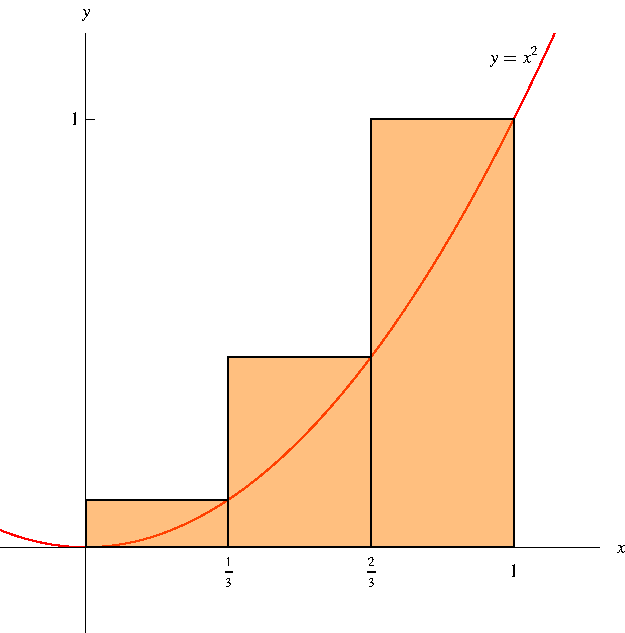
\includegraphics[height=4.2cm]{integration/pictures/05-01-righta.pdf}%
}%
\only<handout:0| 2>{%
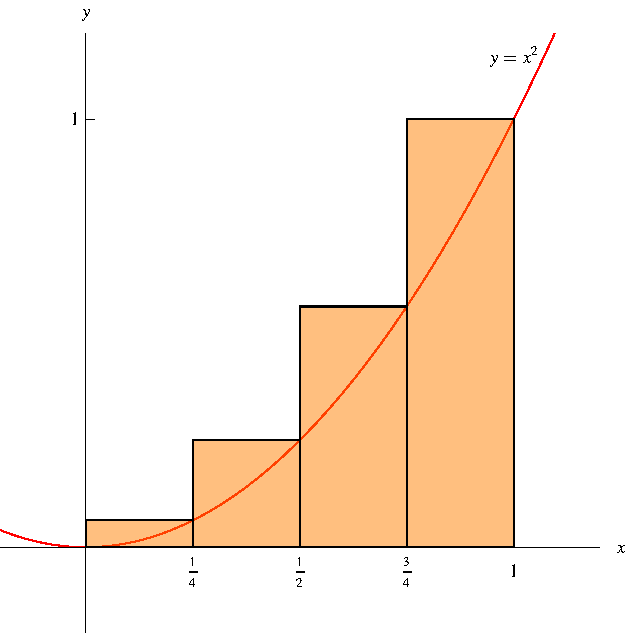
\includegraphics[height=4.2cm]{integration/pictures/05-01-rightb.pdf}%
}%
\only<handout:0| 3>{%
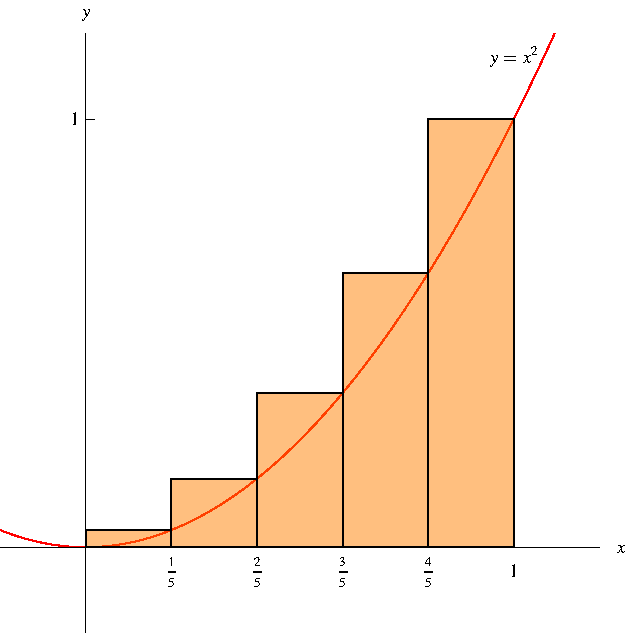
\includegraphics[height=4.2cm]{integration/pictures/05-01-rightc.pdf}%
}%
\only<handout:0| 4>{%
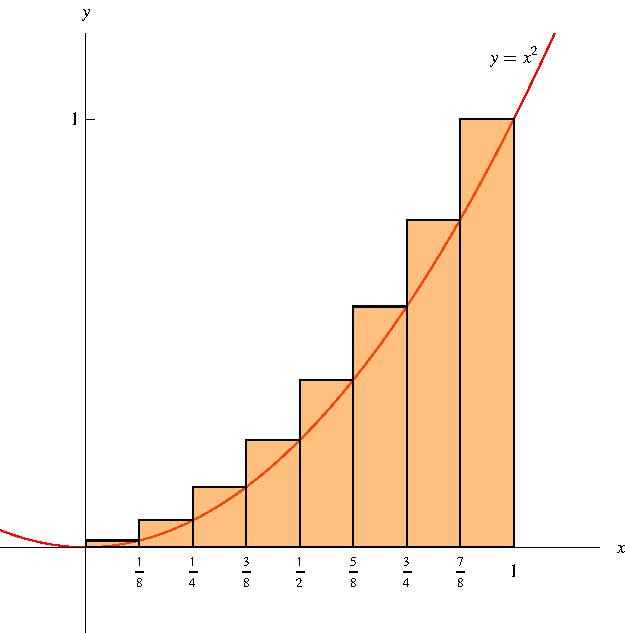
\includegraphics[height=4.2cm]{integration/pictures/05-01-rightd.pdf}%
}%
\only<handout:0| 5>{%
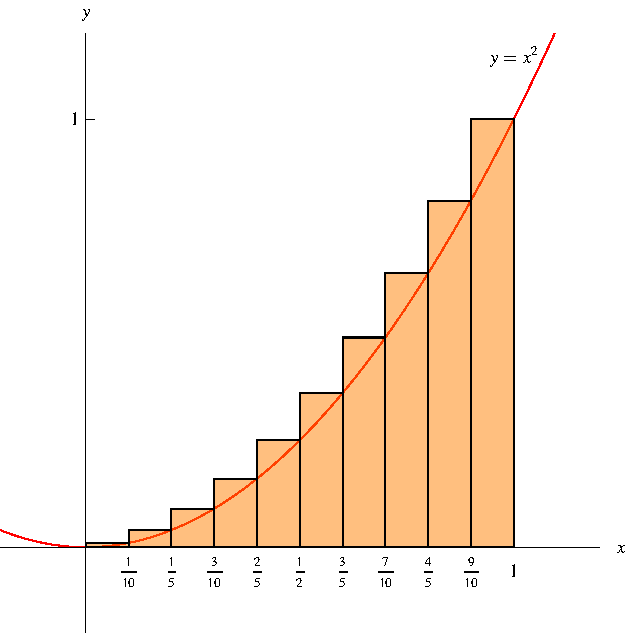
\includegraphics[height=4.2cm]{integration/pictures/05-01-righte.pdf}%
}%
\only<handout:0| 6>{%
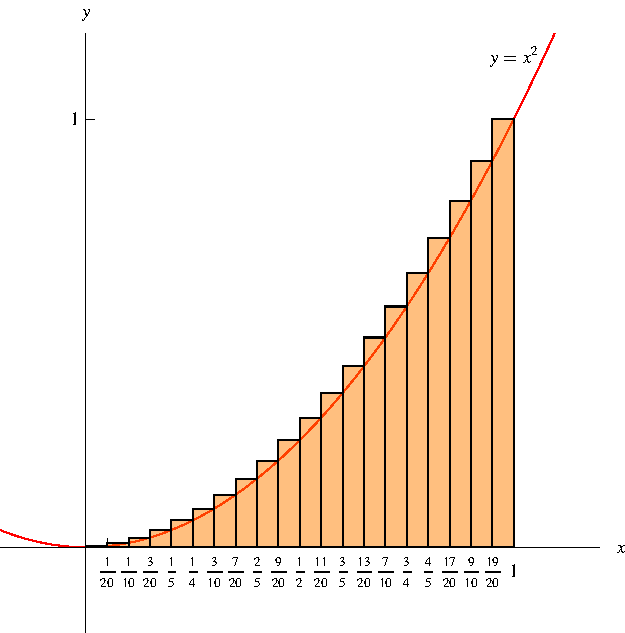
\includegraphics[height=4.2cm]{integration/pictures/05-01-rightf.pdf}%
}%
\only<handout:0| 7>{%
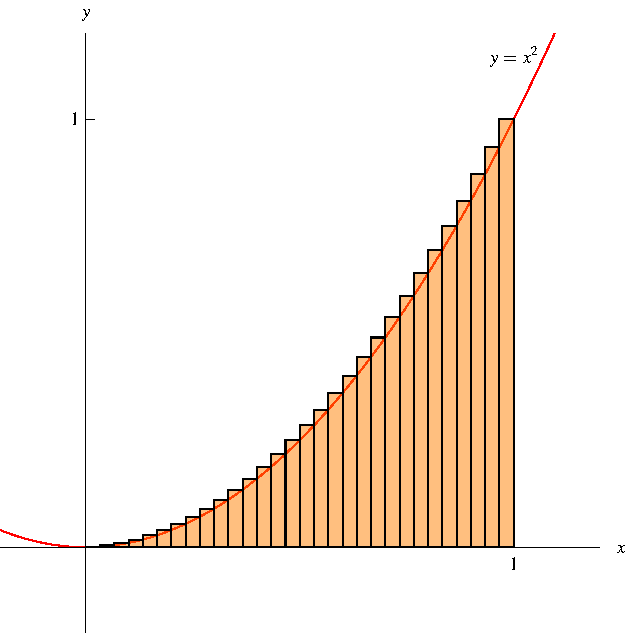
\includegraphics[height=4.2cm]{integration/pictures/05-01-rightg.pdf}%
}%
\only<handout:0| 8>{%
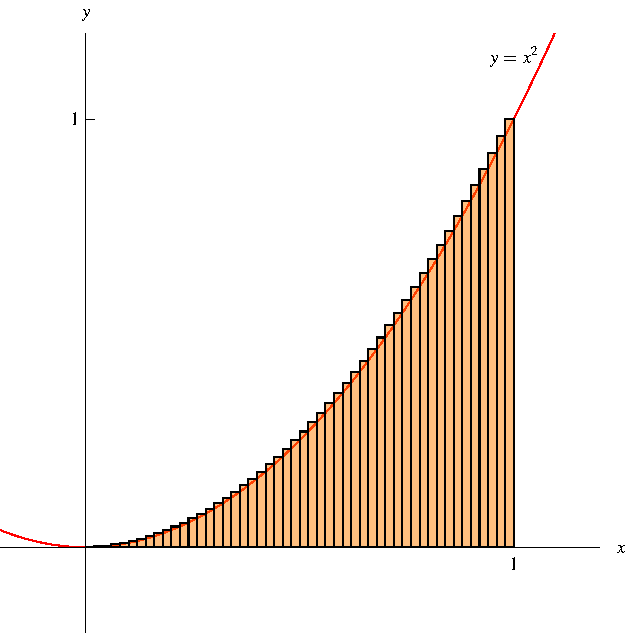
\includegraphics[height=4.2cm]{integration/pictures/05-01-righth.pdf}%
}%
\only<handout:1| 9->{%
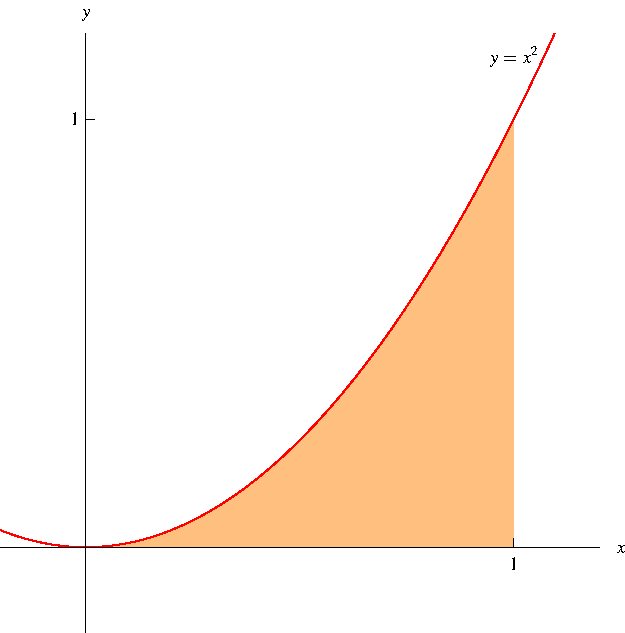
\includegraphics[height=4.2cm]{integration/pictures/05-01-xsquaredarea.pdf}%
}%
\end{columns}
\begin{columns}
\column{.4\textwidth}
\uncover<10->{%
\only<handout:0| -10>{%
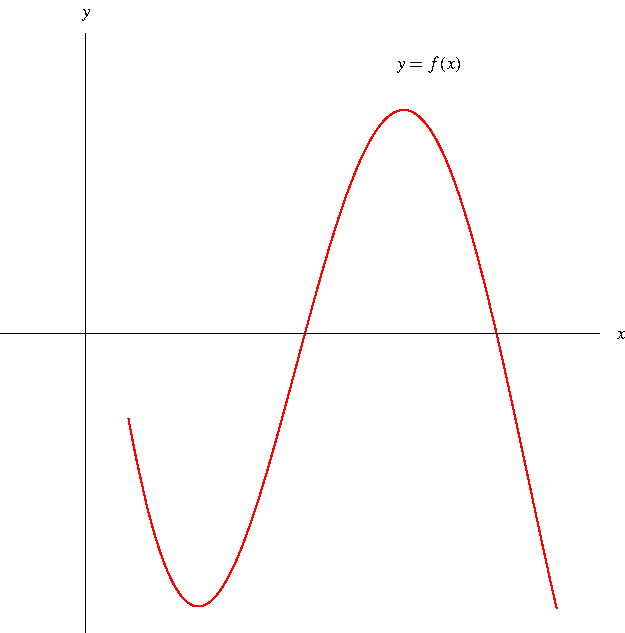
\includegraphics[height=4.2cm]{integration/pictures/05-02-net-area-function.pdf}%
}%
}%
\only<handout:0| 11>{%
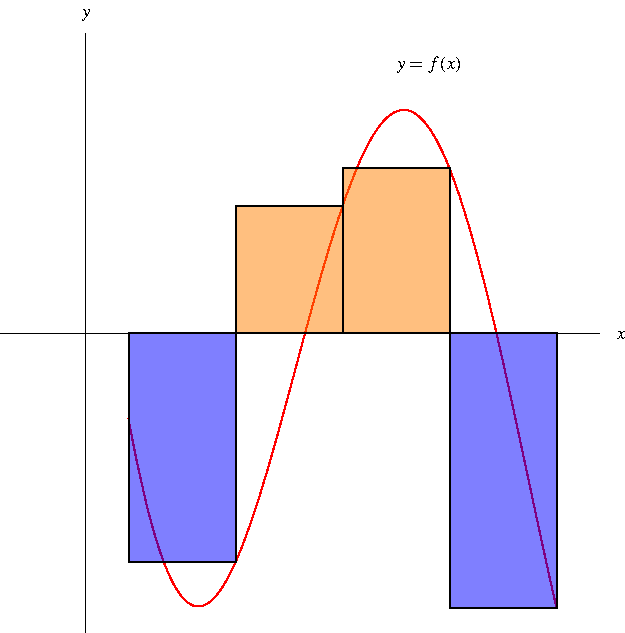
\includegraphics[height=4.2cm]{integration/pictures/05-02-net-areaa.pdf}%
}%
\only<handout:0| 12>{%
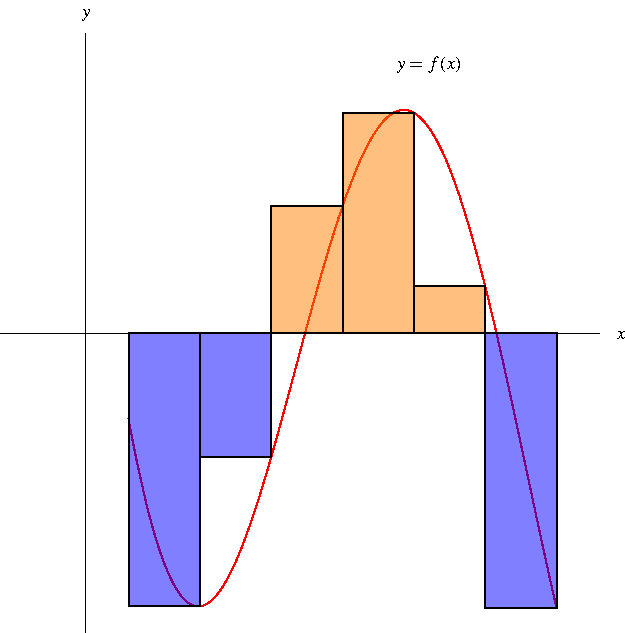
\includegraphics[height=4.2cm]{integration/pictures/05-02-net-areab.pdf}%
}%
\only<handout:0| 13>{%
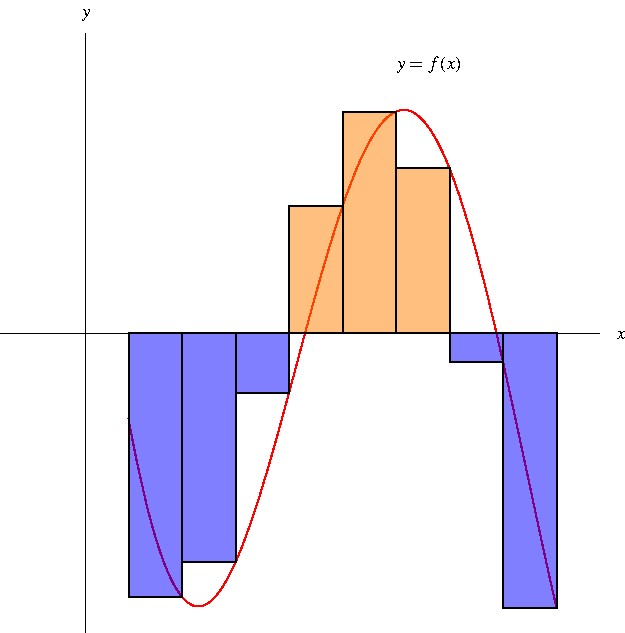
\includegraphics[height=4.2cm]{integration/pictures/05-02-net-areac.pdf}%
}%
\only<handout:0| 14>{%
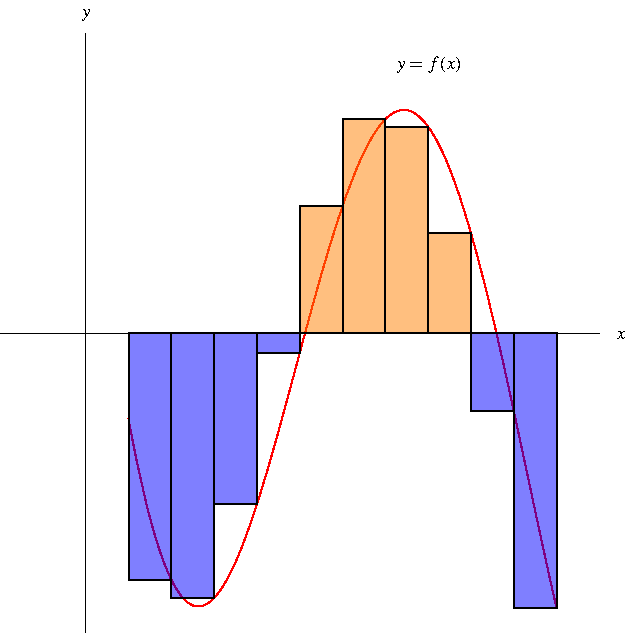
\includegraphics[height=4.2cm]{integration/pictures/05-02-net-aread.pdf}%
}%
\only<handout:0| 15>{%
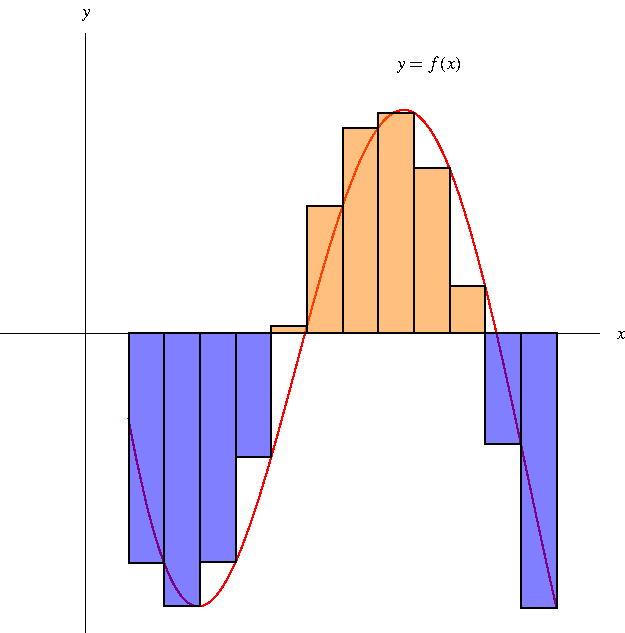
\includegraphics[height=4.2cm]{integration/pictures/05-02-net-areae.pdf}%
}%
\only<handout:0| 16>{%
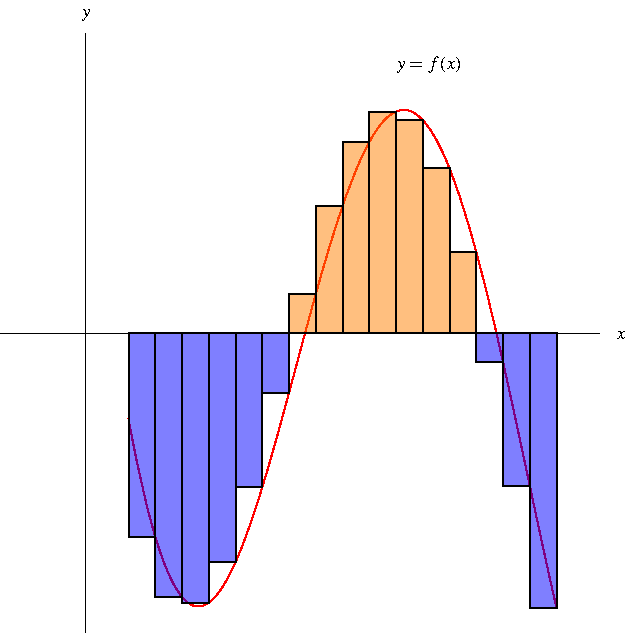
\includegraphics[height=4.2cm]{integration/pictures/05-02-net-areaf.pdf}%
}%
\only<handout:0| 17>{%
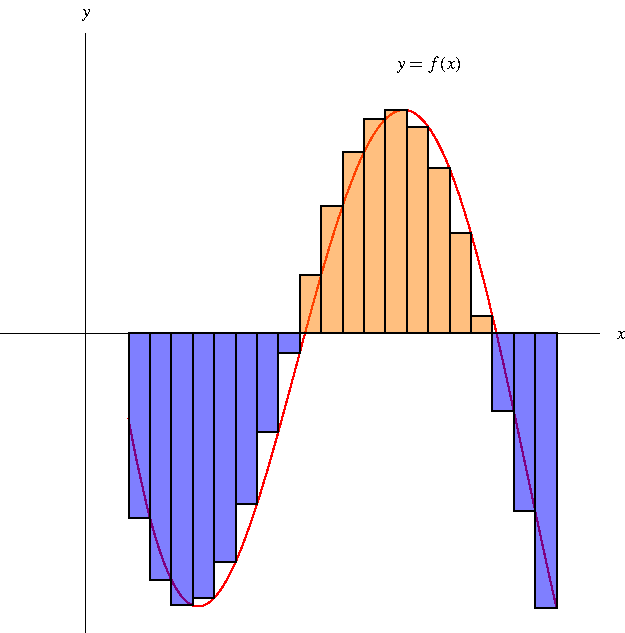
\includegraphics[height=4.2cm]{integration/pictures/05-02-net-areag.pdf}%
}%
\only<handout:0| 18>{%
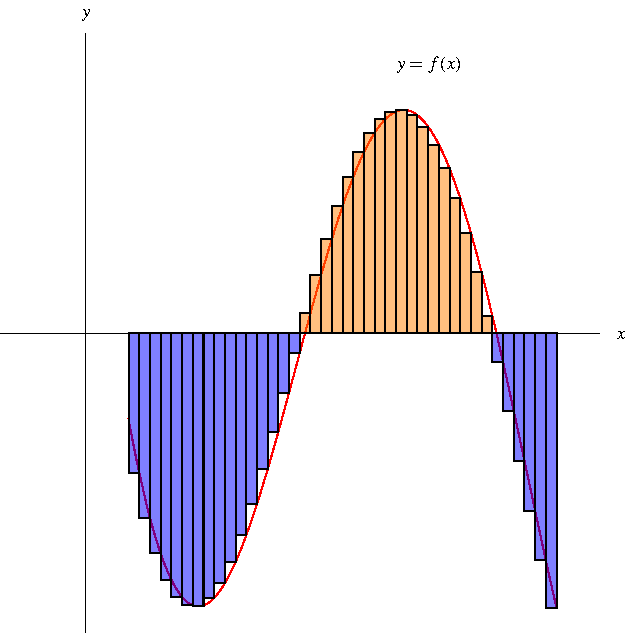
\includegraphics[height=4.2cm]{integration/pictures/05-02-net-areah.pdf}%
}%
\only<handout:1| 19->{%
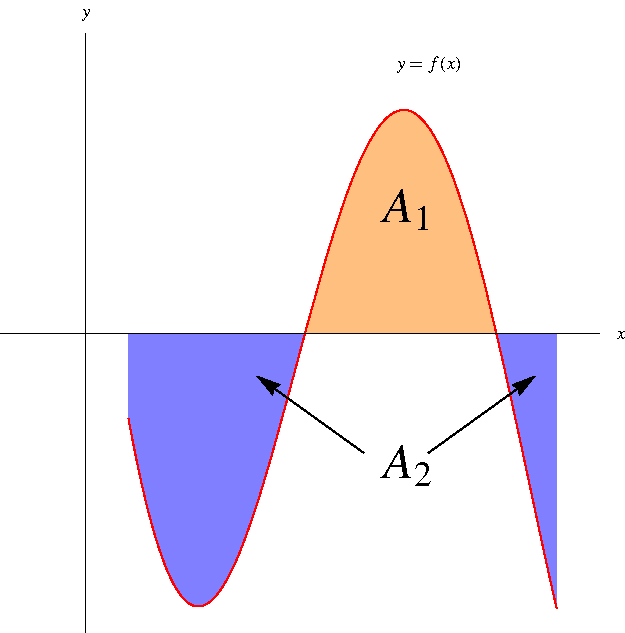
\includegraphics[height=4.2cm]{integration/pictures/05-02-net-area-limit.pdf}%
}%
\column{.6\textwidth}
\begin{itemize}
\item<10->  What if $f(x)$ is sometimes negative?
\item<19->  Then $\int_a^bf(x)\diff x = A_1 - A_2$.
\item<19->  $A_1$ is the area of the region above the $x$-axis and below the graph of $f$.
\item<19->  $A_2$ is the area of the region below the $x$-axis and above the graph of $f$.
\end{itemize}
\end{columns}
\end{frame}
% end module definite-integral-negative
